\documentclass[tikz, border=10pt]{standalone}
\usepackage{helvet}
\usepackage{array}
\renewcommand{\familydefault}{\sfdefault}
\usetikzlibrary{positioning, shapes.multipart, arrows.meta, fit, backgrounds, calc}

\begin{document}
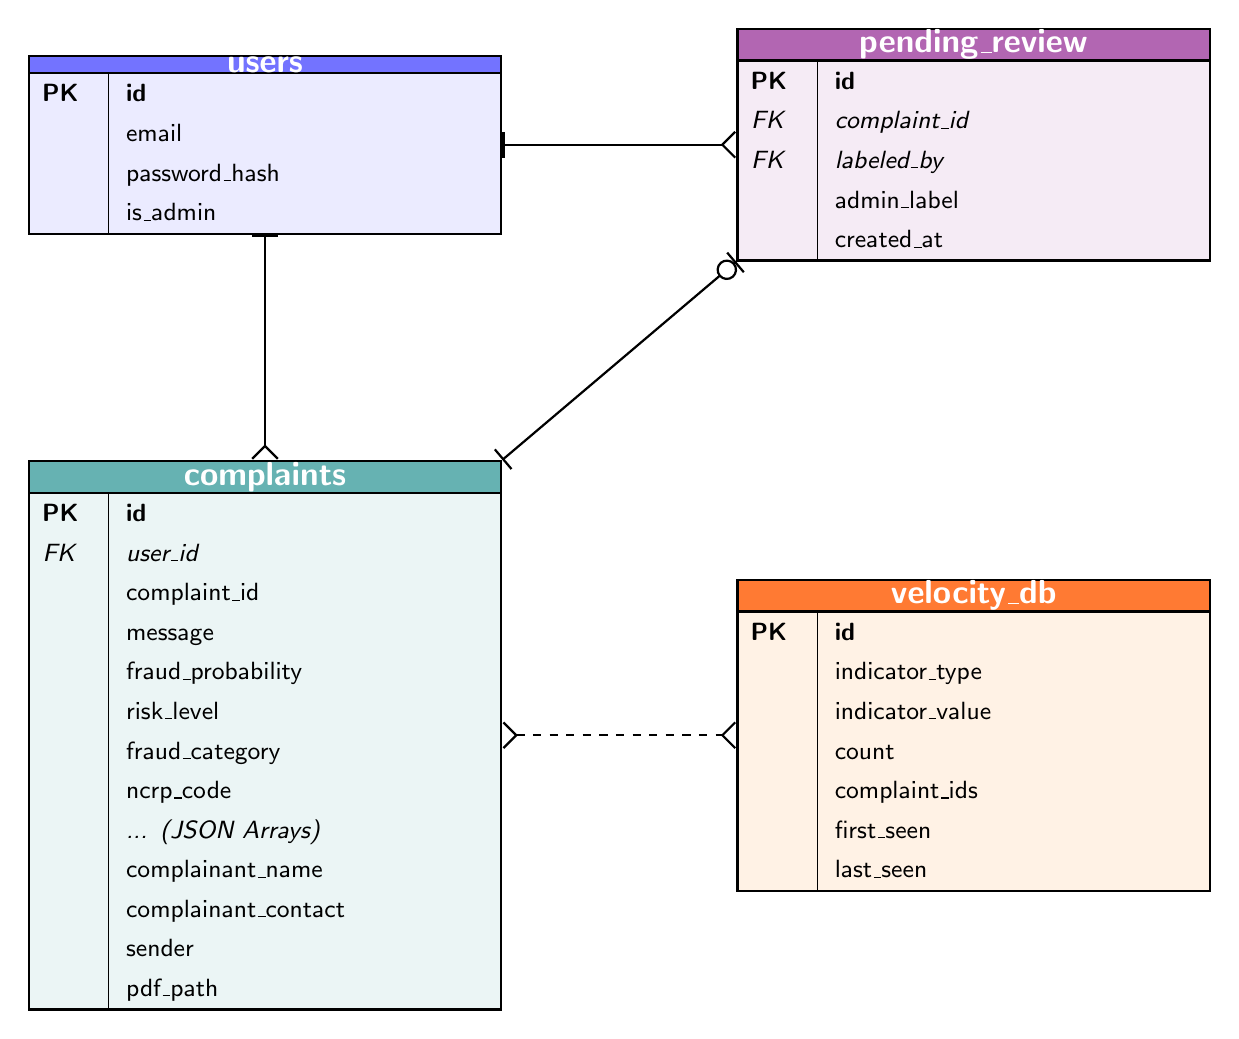
\begin{tikzpicture}[
    table/.style={
        rectangle split,
        rectangle split parts=2,
        draw=black, thick,
        inner sep=0pt,
        text width=6cm,
        align=center,
        font=\small,
        rectangle split part fill={black!20, black!05}
    }
]

% Define a macro for the table body to mimic SS2 exactly (PK column | attribute column)
\newcommand{\tablebody}[1]{%
    \renewcommand{\arraystretch}{1.3}%
    \begin{tabular*}{6cm}{@{} >{\centering\arraybackslash}p{0.8cm} | p{4.8cm} @{}}
        #1
    \end{tabular*}%
}

% Users Table (Top Left) — Blue header
\node[table, rectangle split part fill={blue!55, blue!8}] (users) at (0, 0) {
    \textcolor{white}{\textbf{\large users}}
    \nodepart{second}
    \tablebody{
        \textbf{PK} & \textbf{id} \\
         & email \\
         & password\_hash \\
         & is\_admin \\
    }
};

% Pending Review Table (Top Right) — Purple header
\node[table, rectangle split part fill={violet!60, violet!8}] (pending) at (9, 0) {
    \textcolor{white}{\textbf{\large pending\_review}}
    \nodepart{second}
    \tablebody{
        \textbf{PK} & \textbf{id} \\
        \textit{FK} & \textit{complaint\_id} \\
        \textit{FK} & \textit{labeled\_by} \\
         & admin\_label \\
         & created\_at \\
    }
};

% Complaints Table (Bottom Left) — Teal header
\node[table, rectangle split part fill={teal!60, teal!8}] (complaints) at (0, -7.5) {
    \textcolor{white}{\textbf{\large complaints}}
    \nodepart{second}
    \tablebody{
        \textbf{PK} & \textbf{id} \\
        \textit{FK} & \textit{user\_id} \\
         & complaint\_id \\
         & message \\
         & fraud\_probability \\
         & risk\_level \\
         & fraud\_category \\
         & ncrp\_code \\
         & \textit{... (JSON Arrays)} \\
         & complainant\_name \\
         & complainant\_contact \\
         & sender \\
         & pdf\_path \\
    }
};

% Velocity DB Table (Bottom Right) — Orange header
\node[table, rectangle split part fill={orange!70!red!80, orange!10}] (velocity) at (9, -7.5) {
    \textcolor{white}{\textbf{\large velocity\_db}}
    \nodepart{second}
    \tablebody{
        \textbf{PK} & \textbf{id} \\
         & indicator\_type \\
         & indicator\_value \\
         & count \\
         & complaint\_ids \\
         & first\_seen \\
         & last\_seen \\
    }
};

% ================= RELATIONSHIPS =================
% SS3 Cardinality styles
% 1:N = Bar to Crow's Foot
% 1:0..1 = Bar to Circle-Bar
% N:M = Crow's Foot to Crow's Foot

% 1. Users to Complaints (1 : N) -> Vertical down
\draw[{|[scale=1.5]}-{Straight Barb[reversed, scale=1.5]}, thick] 
    (users.south) -- (complaints.north);

% 2. Users to Pending Review (1 : N) -> Horizontal right
\draw[{|[scale=1.5]}-{Straight Barb[reversed, scale=1.5]}, thick] 
    (users.east) -- (pending.west);

% 3. Complaints to Pending Review (1 : 0..1) -> Diagonal up-right
\draw[{|[scale=1.5]}-{Circle[open, fill=white, scale=1.5] |[scale=1.5]}, thick] 
    (complaints.north east) -- (pending.south west);

% 4. Complaints to Velocity DB (N : M) -> Horizontal right
\draw[{Straight Barb[reversed, scale=1.5]}-{Straight Barb[reversed, scale=1.5]}, thick, dashed] 
    (complaints.east) -- (velocity.west);

\end{tikzpicture}
\end{document}
